\documentclass[12pt]{article}
\usepackage{scrextend}
\usepackage[utf8]{inputenc}
\usepackage[polish]{babel}
\usepackage[T1]{fontenc}%polskie znaki
\usepackage[utf8]{inputenc}%polskie znaki
\usepackage{geometry}
\usepackage{float}
\usepackage{enumitem}
\usepackage{hyperref}
\usepackage{graphicx}
\usepackage{tabulary}
\usepackage{etoc}
\usepackage[normalem]{ulem} 
\renewcommand{\baselinestretch}{1.5}
\graphicspath{ {img/} }
\newgeometry{lmargin=2cm, rmargin=2cm, tmargin=2cm, bmargin=2cm}
\usepackage{tikz}
\usepackage[bf]{caption}
\newcommand{\scenario}[5]{
  \subsection{#1}
  \begin{minipage}{\textwidth}
    \textbf{Cel:} #2 \\
    \textbf{WS:} #3 \\
    \textbf{WK:} #4 \\
    \textbf{Przebieg:}
    \begin{enumerate}
      \setlength\itemsep{0.0em}
      #5
    \end{enumerate}
  \end{minipage}
}

\begin{document}

\begin{flushleft}
        Damian Koper, \textbf{241292} \\
        Łukasz Handschuh, \textbf{241402}
\end{flushleft}
\vspace{1cm}
{
    \centering
    {\Huge\scshape\bfseries Inżynieria oprogramowania - Etap 2 }\\
    \vspace{0.25cm}
    \Large\textbf{Dział ewidencji ludności} \\
    \vspace{0.25cm}
    \large Specyfikacja wymagań funkcjonalnych za pomocą diagramu
    przypadków użycia.\\
}

\section{Wymagania funkcjonalne}

\subsection{Pracownicy}
\begin{enumerate}
    \item Pracownik może zalogować się na swoje konto i z niego się wylogować.
    \item Pracownik z rolą administratora może zarządzać kontami użytkowników.
    \begin{enumerate}
        \item Administrator może stworzyć konto użytkownika.
        \item Administrator może edytować dane i jego rolę użytkownika.
        \item Administrator może usunąć konto użytkownika.
    \end{enumerate}
\end{enumerate}
\subsection{Zarządzanie wnioskami}
\begin{enumerate}
    \item Pracownik może wyświetlić dane wniosków.
    \begin{enumerate}
        \item Pracownik może wyświetlić wnioski tylko danego typu.
        \item Pracownik może wyszukać wniosek podając nr. PESEL.
    \end{enumerate}
    \item Pracownik może wprowadzić wniosek meldunkowy.
    \begin{enumerate}
        \item Pracownik może wprowadzić wniosek o typie \textit{stały} lub \textit{czasowy}.
    \end{enumerate}
    \item Pracownik może edytować dane wniosku meldunkowego.
    \begin{enumerate}
        \item Pracownik może zmienić status wniosku - zaakceptować, lub odrzucić po podaniu powodu.
        \item Zaakceptowany wniosek zmienia się w rekord meldunku.
    \end{enumerate}
    \item Wniosek, by być możliwym do zaakceptowania, musi zawierać komplet danych, które zgadzają się z danymi z systemu PESEL.
\end{enumerate}
\subsection{Zarządzanie meldunkami}
\begin{enumerate}
    \item Pracownik może wyświetlić dane meldunków.
    \begin{enumerate}
        \item Pracownik może wyświetlić dane meldunków tylko danego typu.
        \item Pracownik może wyszukać dane meldunku podając nr. PESEL.
    \end{enumerate}
    \item Pracownik może edytować dane meldunków.
    \begin{enumerate}
        \item Pracownik może zmienić status meldunku na przeszły.
    \end{enumerate}
\end{enumerate}
\section{Wymagania niefunkcjonalne}
\begin{enumerate}
    \item Wszyscy użytkownicy, którzy mają dostęp do aplikacji (posiadają indywidualne konto) mają uprawnienia do edycji danych meldunkowych.
    \item Rola administratora pozwala na zarządzanie użytkownikami i ich uprawnieniami.
    \item System rejestruje historię wszystkich zmian danych meldunkowych.
    \item Dane przesyłane pomiędzy aplikacją, a systemem PESEL są szyfrowane.
    \item W przypadku braku łączności z systemem PESEL pracownik otrzymuje ostrzeżenie o tym fakcie.
    \item Podstawowym źródłem dostępu do danych jest aplikacja internetowa.
    \item Aplikacja umożliwia dostęp do danych przez podstawowy interface konsoli.
\end{enumerate}
\newpage

\section{Aktorzy}

\begin{figure}[!h]
    \centering
    \begin{tabular}{|r|p{5cm}|p{9cm}|}
        \hline
        \textbf{Aktor} & \textbf{Opis} & \textbf{Przypadki użycia} \\
        \hline
        Administrator & 
        Administrator, poza zwykłymi uprawnieniami, ma możliwość zarządzania kontami pracowników.
        & 
        \begin{itemize}
            \setlength\itemsep{-0.5em}
            \item Wszystkie przypadki użycia zdefiniowane dla Pracownika.
            \item PU \nameref{Stworzenie konta pracownika}
            \item PU \nameref{Edycja konta pracownika}
            \item PU \nameref{Usunięcie konta pracownika}
        \end{itemize}
        \\
        \hline
        Pracownik & 
        Pracownik może obsługiwać process dodawania i przetwarzania wniosków meldunkowych, oraz zarządzać istniejącymi meldunkami.
        & 
        \begin{itemize}
            \setlength\itemsep{-0.5em}
            \item PU \nameref{Zalogowanie}
            \item PU \nameref{Wylogowanie}
            \item PU \nameref{Dodanie wniosku} powiącany przez \textit{<<include>>} z PU \nameref{Sprawdzenie poprawności danych}
            \item PU \nameref{Edycja danych wniosku} powiącany przez \textit{<<include>>} z PU \nameref{Sprawdzenie poprawności danych}
            \item PU \nameref{Zmiana statusu wniosku} powiącany przez \textit{<<extend>>} z PU \nameref{Edycja danych wniosku}
            \item PU \nameref{Wyświetlanie wniosków}
            \item PU \nameref{Zmiana kryterium wyświetlania wniosków} powiącany przez \textit{<<extend>>} z PU \nameref{Wyświetlanie wniosków}
            \item PU \nameref{Dodanie meldunku} powiącany przez \textit{<<extend>>} z PU \nameref{Zmiana statusu wniosku}
            \item PU \nameref{Wyświetlanie meldunków}
            \item PU \nameref{Zmiana kryterium wyświetlania meldunków} powiącany przez \textit{<<extend>>} z PU \nameref{Wyświetlanie meldunków}
            \item PU \nameref{Edycja danych meldunku} powiącany przez \textit{<<include>>} z PU \nameref{Sprawdzenie poprawności danych}

        \end{itemize}
        \\
        \hline
    \end{tabular}
    \caption{Opis aktorów wraz z przypisanymi przypadkami użycia.}
\end{figure}

\newpage
\section{Diagram przypadków użycia}
\begin{figure}[h]
    \centering
    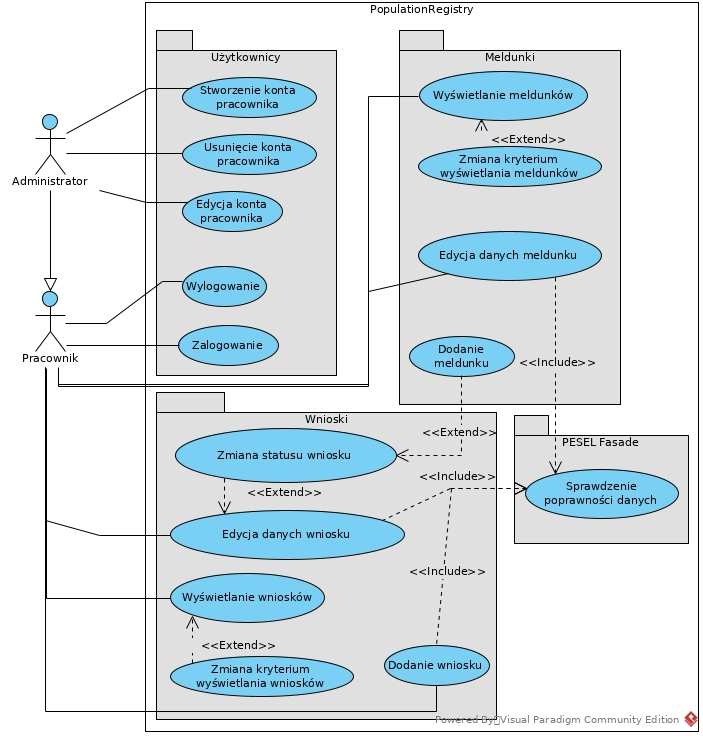
\includegraphics[
        keepaspectratio,
        width=\linewidth,
        height=\dimexpr\textheight-9\baselineskip
    ]{./../paragidm/export/PopulationRegistry_UC.jpg}
    \caption{Diagram przypadków użycia}
    \label{}
\end{figure}

\section{Scenariusze przypadków użycia}

\scenario
    {Stworzenie konta pracownika}
    {Stworzenie nowego konta pracownika.}
    {Inicjalizacja przez uruchomienie programu.}
    {Dodanie nowego konta o unikatowym nr ID i danych osobowych pracownika, lub wyświetlenie komunikatu o błędzie.}
    {
        \item Należy podać dane osobowe pracownika.
        \item Jeśli podane dane są poprawne, można utworzyć konto z nowym nr ID, w przeciwnym razie administrator jest informowany o błędzie.
    }
\scenario
    {Usunięcie konta pracownika}
    {Usunięcie konta pracownika.}
    {Inicjalizacja przez uruchomienie programu.}
    {Usunięcie wybranego konta pracownika.}
    {
        \item Należy podać dane osobowe powiązane z kontem pracownika.
        \item Jeśli odnalezione zostanie konto administrator jest pytany o zatwierdzenie akcji.
        \item Konto jest usuwane, lub akcja zostaje anulowana.
    }
\scenario
    {Edycja konta pracownika}
    {Zmiana danych, lub uprawnień pracownika.}
    {Inicjalizacja przez uruchomienie programu.}
    {Wprowadzenie zmian danych osobowych oraz uprawnień pracownika, lub wyświetlenie komunikatu o błędzie.}
    {
        \item Należy podać nowe dane oraz uprawnienia pracownika.
        \item Jeśli podane dane są poprawne, zostaną zmienione w systemie, w przeciwnym razie administrator jest informowany o błędzie.
    }
\scenario
    {Zalogowanie}
    {Zalogowanie się na konto.}
    {Inicjalizacja przez uruchomienie programu.}
    {Zalogowanie użytkownika do systemie, lub wyświetlenie komunikatu o błędzie.}
    {
        \item Należy podać nazwę użytkownika i hasło.
        \item Jeśli podana nazwa użytkownika i hasło są prawidłowe, następuje zalogowanie do systemu, w przeciwnym razie użytkownik jest informowany o błędzie podczas logowania.
    }
\scenario
    {Wylogowanie}
    {Wylogawanie się z konta.}
    {Użytkownik jest zalogowany w systemie. }
    {Użytkownik jest wylogowany z systemu.}
    {
        \item Należy nacisnąć przycisk wyloguj.
        \item Następuje wylogowanie z systemu.
    }
\scenario
    {Dodanie wniosku}
    {Wstawienie nowego rekordu dotyczącego wniosku meldunkowego.}
    {Inicjalizacja przez uruchomienie programu.}
    {Dodawanie nowego wniosku meldunkowego do bazy, lub wyświetlenie komunikatu o błędzie.}
    {
        \item Należy wprowadzić dane osobowe oraz dane adresowe
        \item Należy wywołać \textit{Sprawdzanie poprawności danych}, które odbędzie się w systemie PESEL.
        \item Jeśli dane okażą się prawidłowe wniosek jest dodawany do bazy, w przeciwnym razie użytkownik jest informowany o błędzie.
    }
\scenario
    {Edycja danych wniosku}
    {Zmiana danych dotyczących wniosku.}
    {Inicjalizacja przez uruchomienie programu.}
    {Zaktualizowanie danych wniosku, lub wyświetlenie komunikatu o błędzie.}
    {
        \item Należy wprowadzić nowe dane osobowe oraz nowe dane adresowe, lub zmienić status wniosku.
        \item Jeśli status zostanie zmieniony należy wywołać \textit{Zmiana statusu wniosku}
        \item Jeśli dane osobowe, lub dane adresowe zostaną zmienione należy wywołać \textit{Sprawdzanie poprawności danych}, które odbędzie się w systemie PESEL.
        \item Jeśli nowe dane okażą się prawidłowe wniosek jest aktualizowany, w przeciwnym razie użytkownik jest informowany o błędzie.
    }
\scenario
    {Wyświetlanie wniosków}
    {Wyświetlenie wymaganych wniosków.}
    {Inicjalizacja przez uruchomienie programu.}
    {Wyświetlenie wniosków.}
    {
        \item Należy wybrać wyświetlanie wniosków.
        \item Wszystkie wnioski przyporządkowane do danego urzędu zostają wyświetlone.
    }
\scenario
    {Zmiana kryterium wyświetlania wniosków}
    {Zawężenie poszukiwań wniosków.}
    {Musi zostać wywołany z \textit{Wyświetlanie wniosków} .}
    {Wyświetlenie tylko wniosków spełniających kryteria.}
    {
        \item Należy wprowadzić kryteria takie jak PESEL, imię i nazwisko.
        \item Wnioski spełniające podane kryteria są wyświetlane.
    }
\scenario
    {Zmiana statusu wniosku}
    {Odrzucenie, lub zaakceptowanie wniosku.}
    {Musi zostać wywołana z \textit{Edycja danych wniosku}.}
    {Wniosek zostaje odrzucony, lub zaakceptowany.}
    {
        \item Należy zmienić wniosku na odrzucony, lub zaakceptowany.
        \item Jeśli wniosek został zaakceptowany należy wywołać \textit{Dodanie meldunku}.
    }
\scenario
    {Dodanie meldunku}
    {Wstawienie nowego rekordu dotyczącego meldunku.}
    {Musi zostać wywołane z \textit{Zmiana statusu wniosku}.}
    {Dodanie nowego meldunku do bazy.}
    {
        \item Meldunek zostaje dodany do bazy z obecnym statusem.
        \item Jeśli wnioskujący posiada w bazie inne meldunki aktualizowany jest ich status.
    }
    \scenario
    {Wyświetlanie meldunków}
    {Wyświetlenie wymaganych meldunków.}
    {Inicjalizacja przez uruchomienie programu.}
    {Wyświetlenie meldunków.}
    {
        \item Należy wybrać wyświetlanie meldunków.
        \item Wszystkie meldunki przyporządkowane do danego urzędu zostają wyświetlone.
    }
\scenario
    {Zmiana kryterium wyświetlania meldunków}
    {Zawężenie poszukiwań meldunków.}
    {Musi zostać wywołany z \textit{Wyświetlanie meldunków} .}
    {Wyświetlenie tylko meldunków spełniających kryteria.}
    {
        \item Należy wprowadzić kryteria takie jak PESEL, imię i nazwisko.
        \item Meldunki spełniające podane kryteria są wyświetlane.
    }
\scenario
    {Edycja danych meldunku}
    {Zmiana danych dotyczących meldunku.}
    {Inicjalizacja przez uruchomienie programu.}
    {Dane meldunku są zaktualizowane, lub wyświetlenie komunikatu o błędzie.}
    {
        \item Należy wprowadzić nowe dane osobowe oraz nowe dane meldunkowe.
        \item Należy wywołać \textit{Sprawdzanie poprawności danych}, które odbędzie się w systemie PESEL.
        \item Jeśli nowe dane okażą się prawidłowe meldunek jest aktualizowany, w przeciwnym razie użytkownik jest informowany o błędzie.
    }
\scenario
    {Sprawdzenie poprawności danych}
    {Walidacja danych osobowych.}
    {Może zostać wywołana z \textit{Edycja danych wniosku, Edycja danych meldunku}.}
    {Potwierdzenie poprawności danych.}
    {
        \item Moduł obsługi systemu PESEL sprawdza matematyczną poprawność numeru PESEL.
        \item System PESEL zwraca informacje dotyczącą poprawności danych oraz obecności obywatela w systemie.
    }
\end{document}